\documentclass{article}
\usepackage[utf8]{inputenc}
\usepackage[english]{babel}

% Convenience improvements
\usepackage{csquotes}
\usepackage{enumitem}
\setlist[enumerate,1]{label={\alph*)}}
\usepackage{amsmath}
\usepackage{amssymb}
\usepackage{mathtools}
\usepackage{tabularx}

% Proper tables and centering for overfull ones
\usepackage{booktabs}
\usepackage{adjustbox}

% Change page/text dimensions, the package defaults work fine
\usepackage{geometry}

\usepackage{parskip}

% Drawings
\usepackage{tikz}
\usepackage{pgfplots}
\pgfplotsset{compat=1.18}
\usetikzlibrary{automata,positioning}

% Adjust header and footer
\usepackage{fancyhdr}
\pagestyle{fancy}
\fancyhead[L]{\textbf{Computational Complexity} --- Group Project}
\fancyhead[R]{}
\fancyfoot[C]{}
\fancyfoot[R]{\thepage}
% Stop fancyhdr complaints
\setlength{\headheight}{12.5pt}

\usepackage{hyperref}

\newcommand{\Deltaop}{\, \Delta\, }
\newcommand{\xor}{\, \oplus\, }
\newcommand{\id}{\text{id}}

\begin{document}

\section*{Vertex Cover is NP-complete}

\emph{Jannik Jungmann (12103135), Laurenz Weixlbaumer (11804751)}

A vertex cover of a graph is a set of vertices that includes at leat one endpoint of every edge of the graph\footnote{\url{https://en.wikipedia.org/wiki/Vertex_cover}}. The \textsc{Vertex Cover} problem is: Given a graph $G$ and an integer $k$, does $G$ have a vertex cover of size $\leq k$?

\begin{figure}[htp]
    \centering
    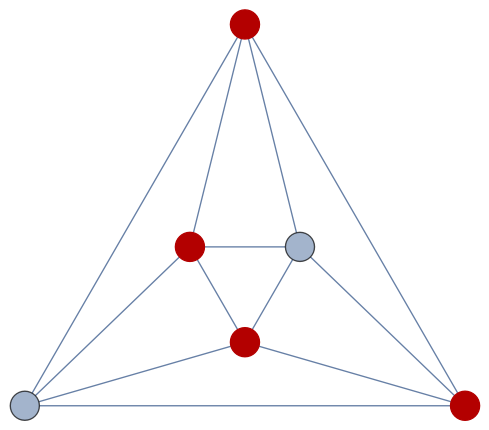
\includegraphics[width=.3\textwidth]{vertex_example_graph_11.png}\qquad
    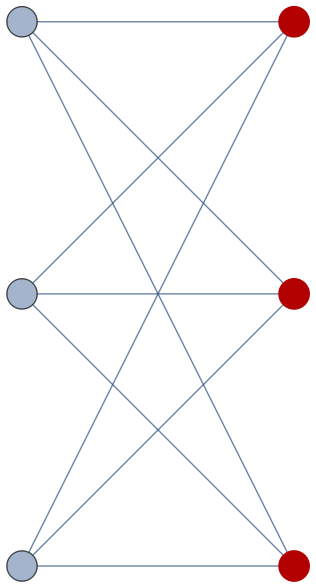
\includegraphics[width=.18\textwidth]{vertex_example_graph_22.png}\qquad
    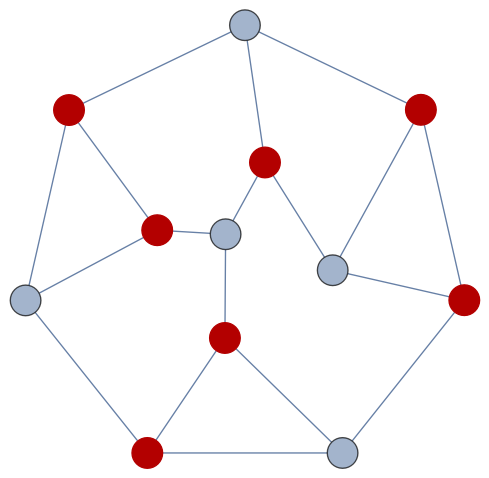
\includegraphics[width=.3\textwidth]{vertex_example_graph_33.png}

    \caption{Various graphs with a highlighted minimum vertex cover.}
\end{figure}

We have chosen this problem for its rich representation in the literature and its reasonably straight\-forward proof of \textbf{NP}-completeness. We will first show that another decision problem, \textsc{Independent Set}, is \textbf{NP}-complete by giving a reduction from 3-SAT, and then demonstrate a simple reduction from it to \textsc{Vertex Cover}. We realize that this is not (exactly) what was required but believe that it is within the spirit of the exercise.

An independent set is a set of vertices in a graph, no two of which are adjacent\footnote{\url{https://en.wikipedia.org/wiki/Independent_set_(graph_theory)}}. The \textsc{Independent Set} problem is: Given a graph $G$ and an integer $k$, does $G$ have an independet set of size $\geq k$?

\paragraph{Lemma} \textsc{Independent Set} is \textbf{NP}-complete.\footnote{See \url{https://www.cs.cmu.edu/~15451-f17/lectures/lec23-np.pdf}, p.5 and \url{http://www.cs.cornell.edu/courses/cs482/2005su/handouts/NPComplete}, p.2.}

We can verify that a given set $S \subset V$ is independent in a graph $G(V, E)$ by checking for all $v_1, v_2 \in S$ that $(v_1, v_2) \not\in V$. This can be done in polytime. We can check that $|S| \geq k$ in constant time. Thus \textsc{Independent Set} is in \textbf{NP}.

We will now reduce from 3-SAT. Let $F$ be an arbitrary instance of 3-SAT with clauses $C_1, \ldots C_k$ in the variables $x_1, \ldots x_n$. We construct the graph $G$ such that it has a triangle (three interconnected nodes) for each clause $C_i$. Nodes of these triangles are labeled with the terms of its clause (either $x_i$ or $\overline{x_i})$. We then add edges between every pair of nodes $(x_i, \overline{x_i})$.

If $F$ is satisfiable there is a true term in each triangle. We pick that node from each triangle, leading to an independent set of size $k$. These nodes are independent because we only picked one node from each triangle, and the only edges between triangles go between nodes with labels $x_i$ and $\overline{x_i}$ (which can't both be satisfied). So if and only if there is a satisifiable assignment, we will find an independent set of size $k$.

\paragraph{Theorem} \textsc{Vertex Cover} is \textbf{NP}-complete.\footnote{See \url{https://www.cs.cmu.edu/~15451-f17/lectures/lec23-np.pdf}, p.5 (again) and \url{http://cs.williams.edu/~shikha/teaching/spring20/cs256/lectures/Lecture22.pdf}, p.17 (goes in the other direction, but still useful as reference).}

We can verify that a given set $S$ covers a graph $G(V, E)$ by checking that for all $(u, v) \in E$ we have either $u \in S$ or $v \in S$ and $|S| \leq k$. This is possible in polytime. Thus \textsc{Vertex Cover} is in \textbf{NP}.

We will reduce from \textsc{Independent Set}. Consider that if $C$ is a vertex cover in a graph $G(V, E)$ then $V \backslash S$ is an independent set -- there cannot be an edge between any two vertices in $V \backslash S$ because otherwise $C$ would not cover all edges. In the same spirit, if $S$ is an independent set then $V \backslash S$ is a vertex cover.

This allows us to transform a given instance $(G, k)$ of \textsc{Independent Set} to an instance $(G, |V| - k)$ for \textsc{Vertex Cover}. This works because we have just established that \enquote{is there an independent set of size $\geq k$} is equivalent to \enquote{is there a vertex cover of size $\leq |V| - k$}.

\end{document}
